In this chapter I present the surface stress and adhesion energy data collected for two types of silicone with various stiffnesses. We first used Gelest to obtain our preliminary data and tune the operation of our device. We then switched to Dow-Corning to continue more extensive measurements. 
\section{Preliminary Data}
\subsection{Standard Candles}
Below (Fig. \ref{fig:190215g91glasssphere011surface}) is a raw data image:
\begin{figure}[h!]
	\centering
	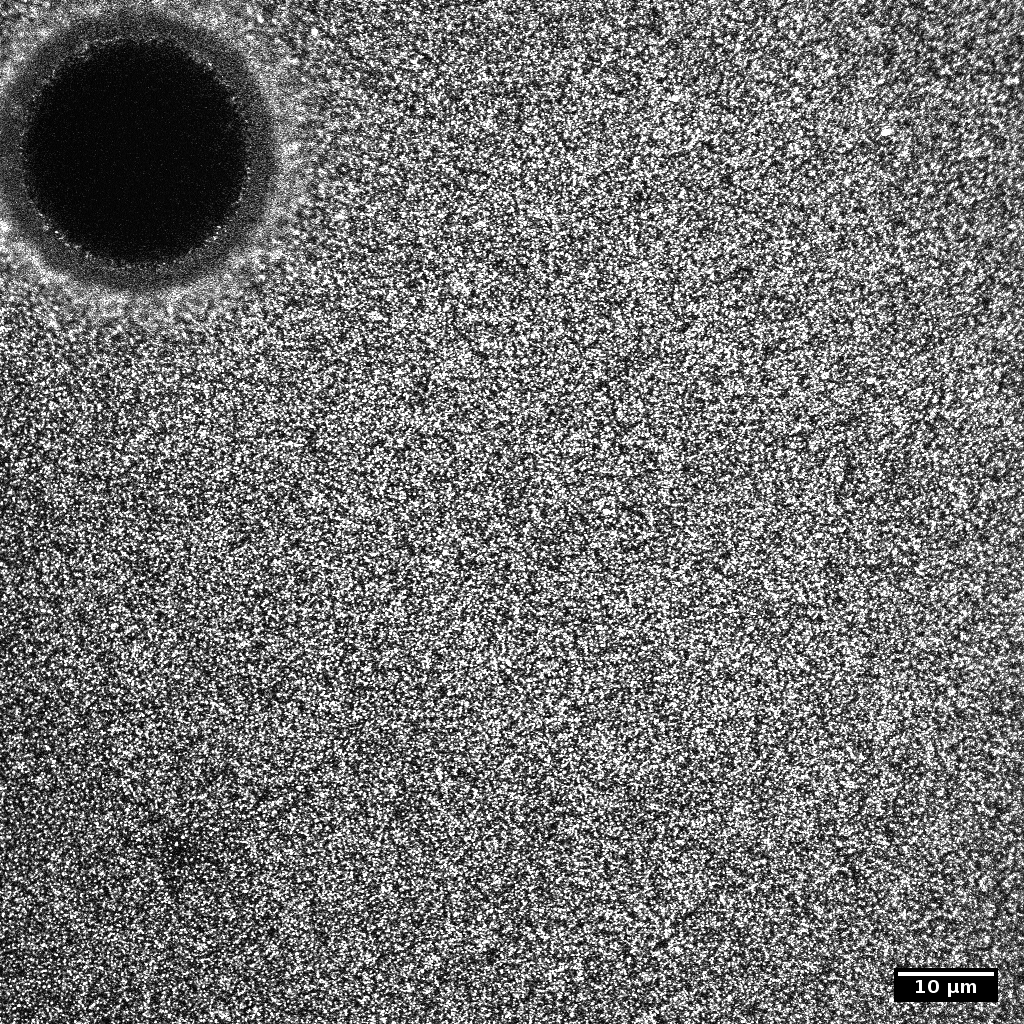
\includegraphics[width=.6\linewidth]{Chapters/Figures/190215_g91_glass_sphere011_surface.png}
	\caption[The surface plane of a silica bead in silcone]{The surface plane of a silica bead in Gelest 9:1 Silicone (E = 7.3 kPa). Radius of sphere = 28.7 $\mu$m.}
	\label{fig:190215g91glasssphere011surface}
\end{figure}

The ``black hole'' like image in the top-left corner is the silica sphere. Each small white dot represents a fluorescent bead; together they create a sea of stars that outline the surface plane and the silica sphere. Figure \ref{fig:190215g91glasssphere011surface} is an example of the upper limit of bead coverage density. Any higher concentration of fluorescent beads could result in a difficulty in light bleeding. Note, the sphere is in the top corner of the image to provide maximum information about the leveling of the surface plane. We assume that the surface effects are symmetrical for zero applied strain and equibiaxial strain. Thus, it is more important to gather information in one direction to properly level the surface plane to determine the depth into which the sphere sinks. 

\emph{Ok, I'm not sure what I want to do with the graphic below, But I know I want it there in some way. Also the lettering could be a place holder. I could give an actual depth in microns for each image.}

\begin{figure}[h!]
	\begin{tabular}{ccc}
		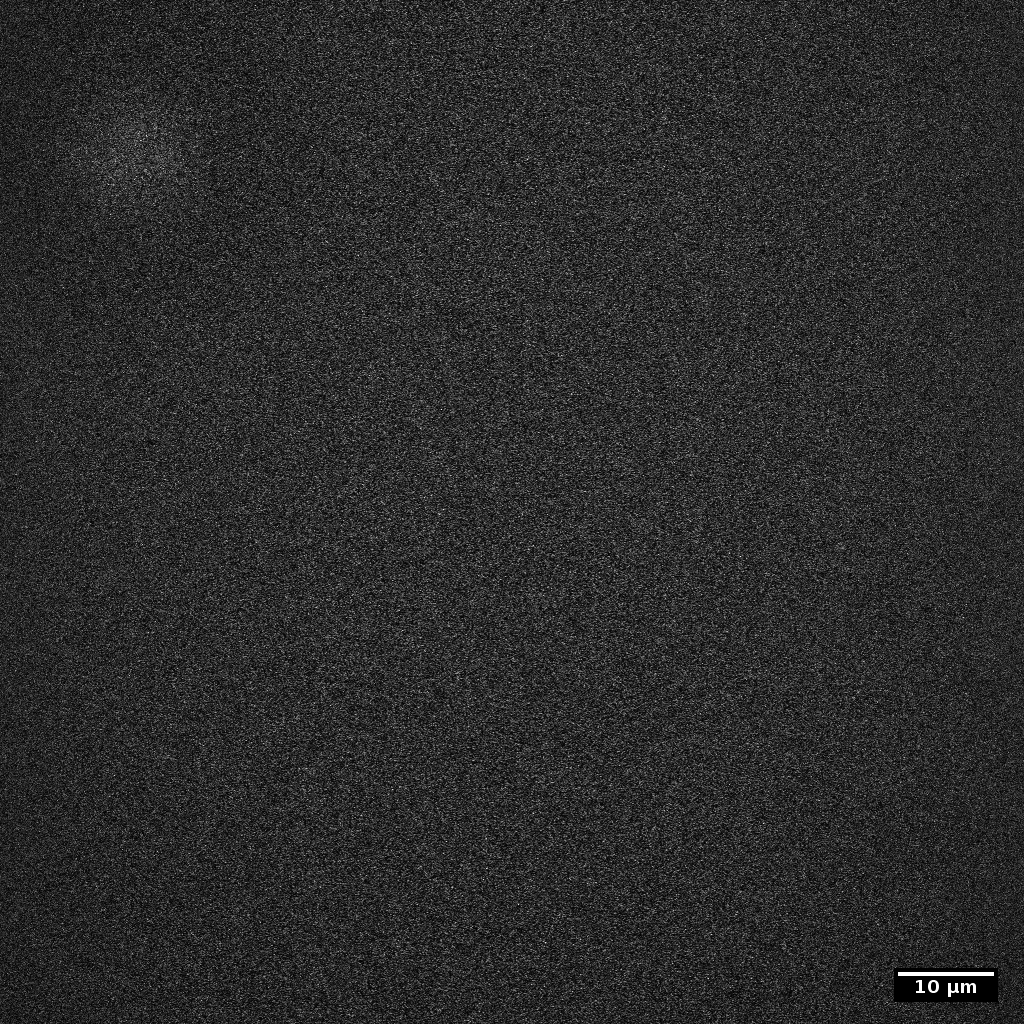
\includegraphics[width= .33\linewidth]{Chapters/Figures/190215_g91_glass_sphere011_cascade1.png} & 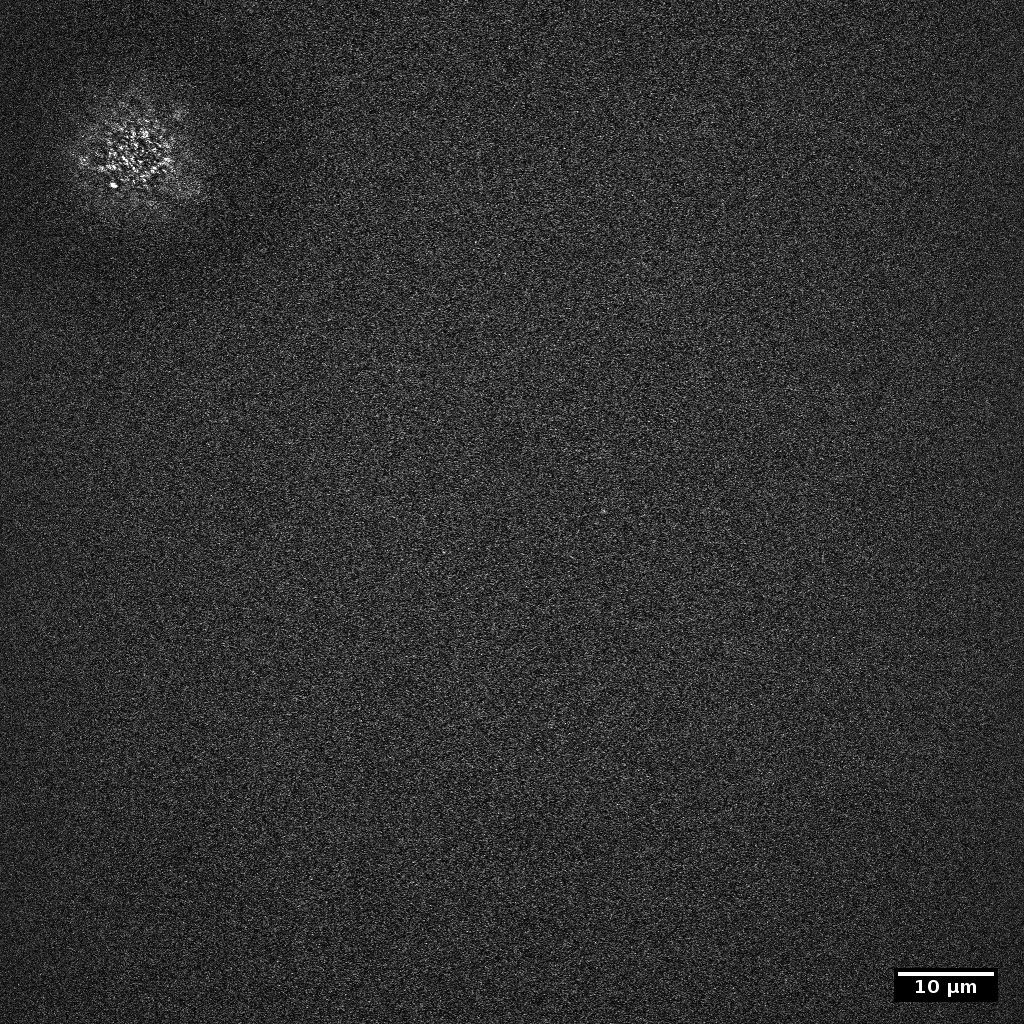
\includegraphics[width= .33\linewidth]{Chapters/Figures/190215_g91_glass_sphere011_cascade2.png} & 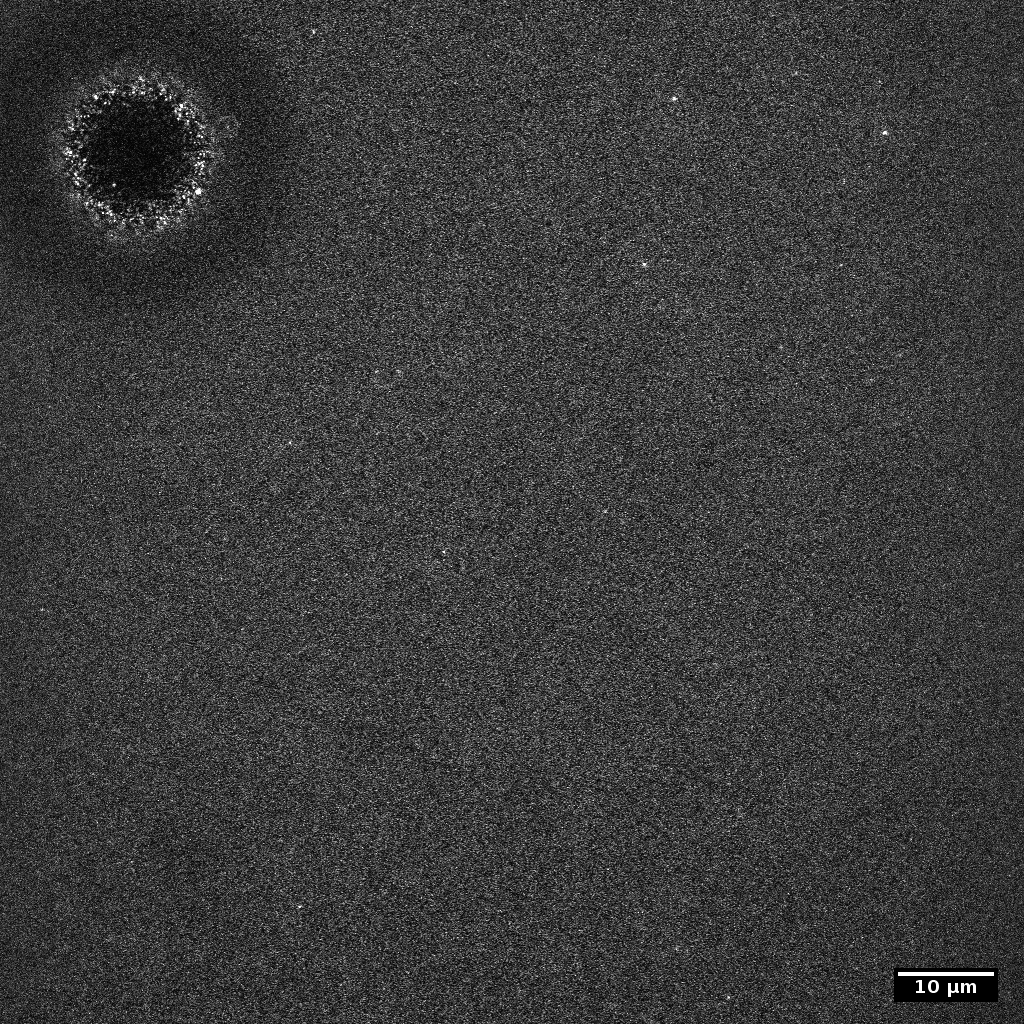
\includegraphics[width= .33\linewidth]{Chapters/Figures/190215_g91_glass_sphere011_cascade3.png} 
		\\
		a) & b) & c) \\
		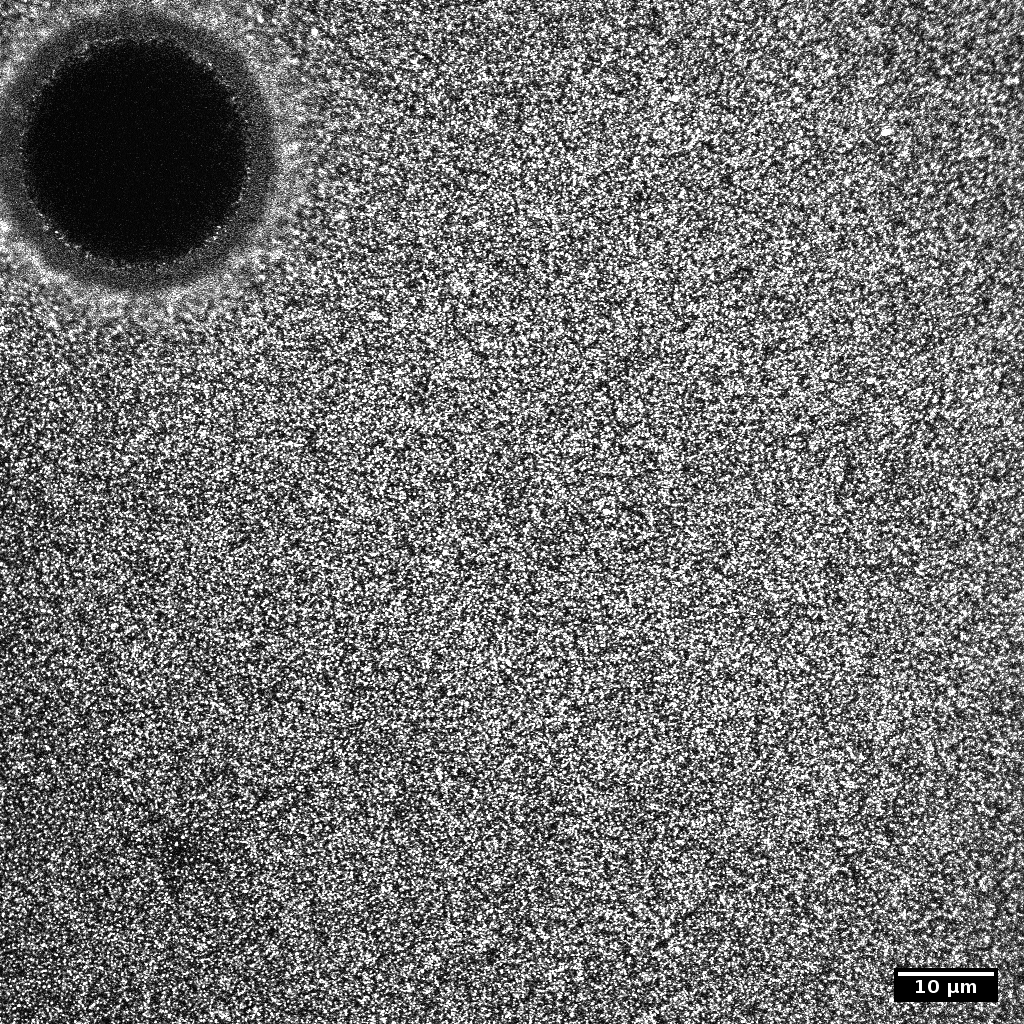
\includegraphics[width= .33\linewidth]{Chapters/Figures/190215_g91_glass_sphere011_cascade4.png} & 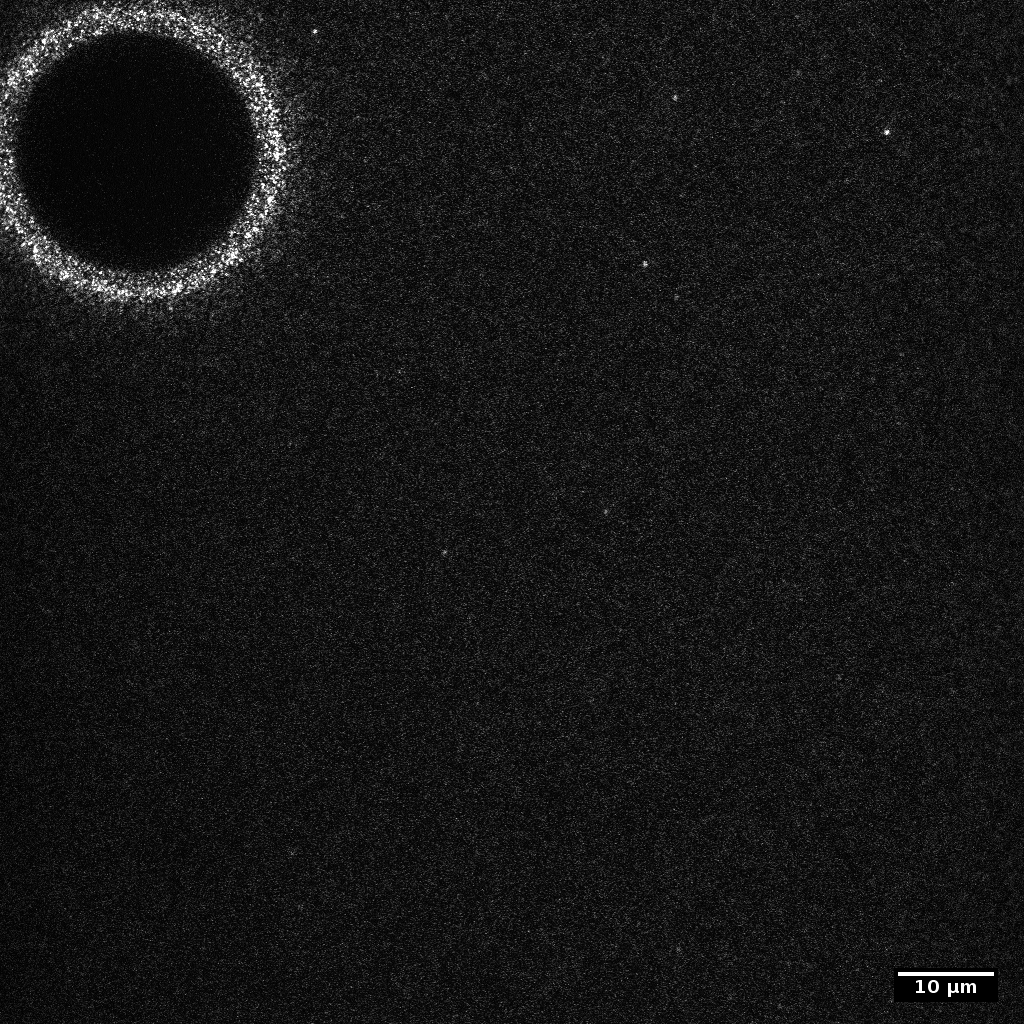
\includegraphics[width= .33\linewidth]{Chapters/Figures/190215_g91_glass_sphere011_cascade5.png} & 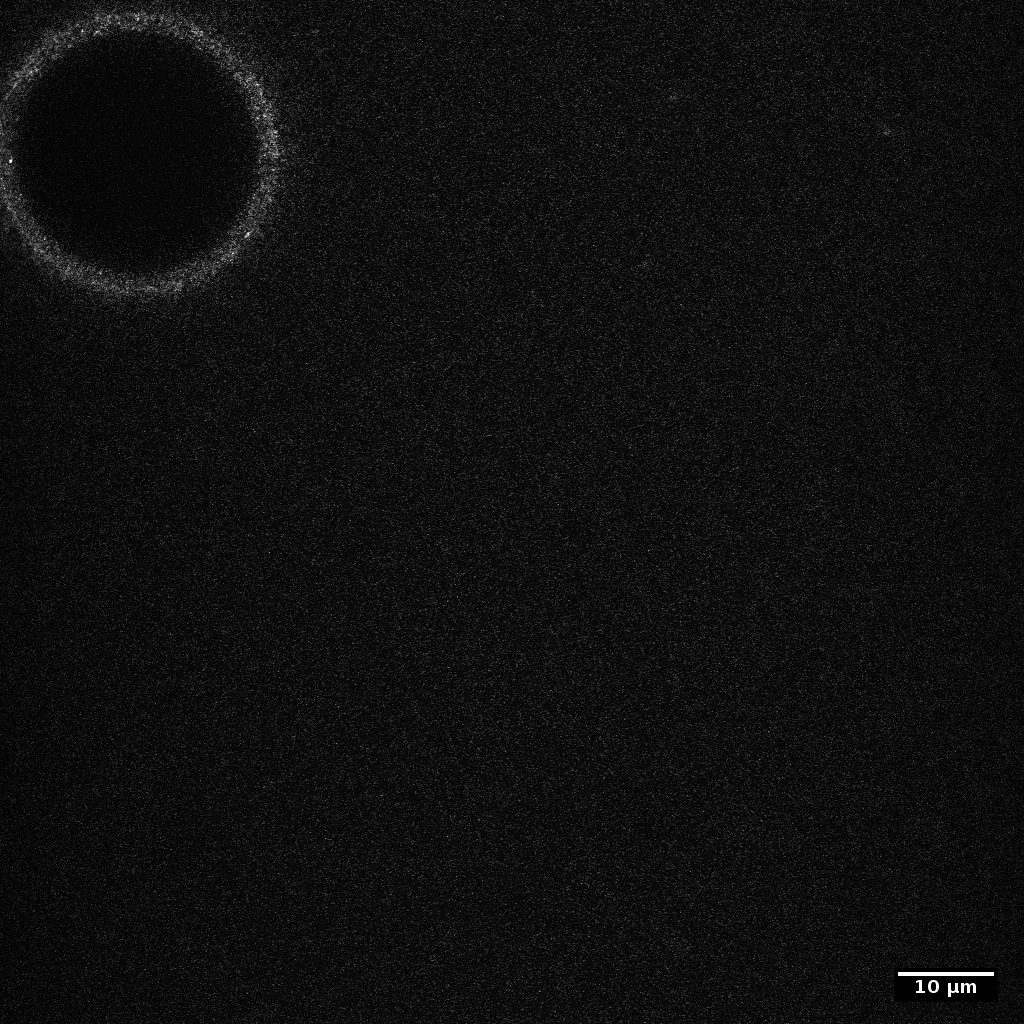
\includegraphics[width= .33\linewidth]{Chapters/Figures/190215_g91_glass_sphere011_cascade6.png}
		\\
		d) & e) & f) 
	\end{tabular}
	\label{fig:sphere011cascade}
	\caption[Vertical path through image stack]{Images a-f display the x-y plane of the same sample traversing vertically from below the silica sphere to above the surface plane. The scale bar in the bottom right corners represent 10 $\mu$m}
\end{figure}

Not only do we measure the depth and radii for a range of spheres, but we also measure a select few spheres at every strain. This allows us to track how any given sphere is changing, increasing our confidence that the shift in $\Upsilon$ and W is not just an artifact of noise. Below is the side profile for Gelest 9:1 ($\text{E}=6.3$ kPa). Notice how the profile shifts noticeably upwards to be flattened when the substrate is stretched. This shift is expected if the surface stress is increasing (see equation \ref{THEeqn}).

\begin{figure}
	\centering
	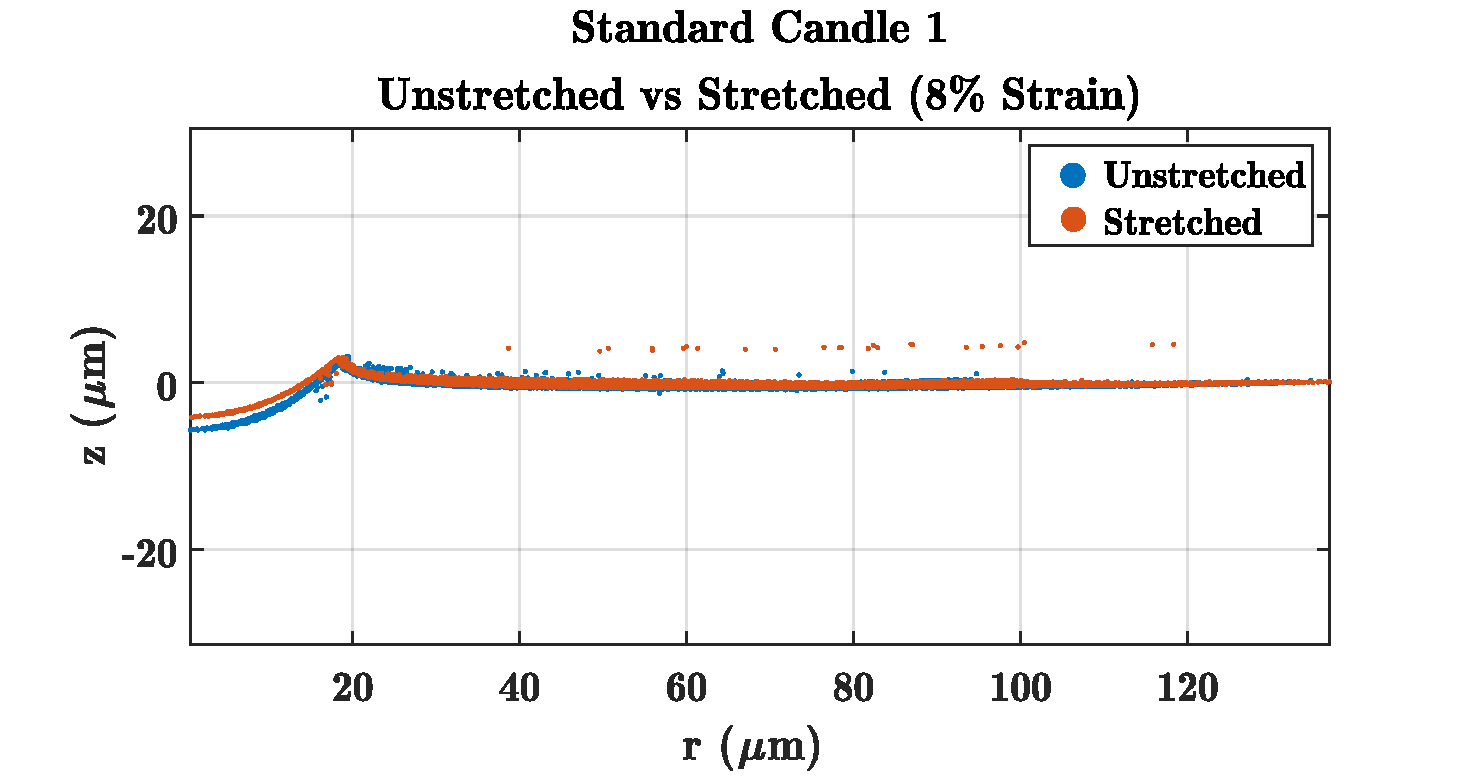
\includegraphics[width=\linewidth]{Chapters/Figures/sc1_unstretched_v_8ml}
	\caption[Side Collapse Comparison]{The side profile of the same sphere before and after stretch. Notice how after stretching, the sphere's indentation into the substrate is shallower. Substrate is Gelest 9:1 ($\text{E}=6.3$ kPa).}
	\label{fig:sc1unstretchedv8ml}
\end{figure}

\section{Data}
\emph{go get that sweet DC d vs r goodness}